\documentclass[frame number]{beamer}
\usepackage[utf8]{inputenc}
\usepackage{amsmath}
\usepackage{hhline}
\usepackage{tikz}
\usepackage{xcolor,colortbl}
\usetikzlibrary{arrows,decorations,matrix,positioning,fit}

\tikzset{%
  post/.style={rectangle,draw=blue!70,top color=white,bottom color=blue!20,very thick},
  user/.style={circle,top color=white,draw=red!70,bottom color=red!20,very thick},
  plain/.style={rectangle,draw=black!70,top color=white, bottom color=black!20,very thick}%
}

\usetheme{Ilmenau}

%% META DATA
\title{Interesting Content and User Discovery without Upvotes}
\subtitle{An application of centrality measures to Reddit}
\author{Rollen S. D'Souza \\ {\texttt{rollen.dsouza@uwaterloo.ca}}}
\institute{University of Waterloo}
\date{2018}

\begin{document}

\frame{\titlepage}

%% OUTLINE
\begin{frame}
  \frametitle{Outline}
  \tableofcontents
\end{frame}

%% INTRODUCTION
\section{Introduction}
\subsection{About Reddit}

\begin{frame}
  \frametitle{What is Reddit?}
  \framesubtitle{Purposes}
  \begin{itemize}
    \item<1->{Social news aggregation}
    \item<2->{Discussion platform}
    \item<3->{Community for help or relaxation}
  \end{itemize}
\end{frame}

\begin{frame}
  \frametitle{What is Reddit?}
  \framesubtitle{Basic Structure}
  \begin{figure}
    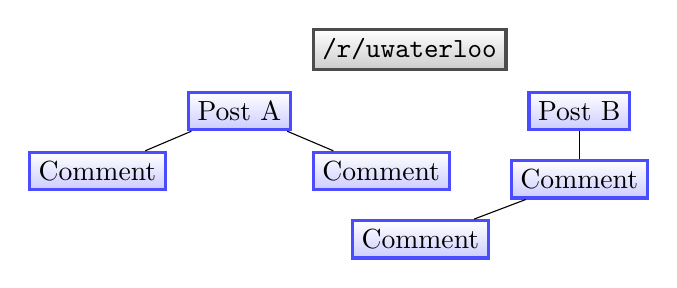
\begin{tikzpicture}[node distance=1em]
      \node (subreddit) [plain] {\texttt{/r/uwaterloo}};
      \node (post_a) [post, below left=of subreddit] {Post A};
      \node (post_b) [post, below right=of subreddit] {Post B};
      \node (comment_1) [post,below left=of post_a] {Comment};
      \node (comment_2) [post,below right=of post_a] {Comment};
      \node (comment_3) [post,below = of post_b] {Comment};
      \node (comment_4) [post,below left=of comment_3] {Comment};

      \path (post_a) edge[-] (comment_1)
            (post_a) edge[-] (comment_2);
      \path (post_b) edge[-] (comment_3) (comment_3) edge[-] (comment_4);

    \end{tikzpicture}
    \caption{Graph-like structure of the Reddit platform.}
    \label{fig:reddit:graph}
  \end{figure}
\end{frame}

\begin{frame}
  \frametitle{What is Reddit?}
  \begin{center}
    
\includegraphics[height=0.85\textheight, keepaspectratio=true]{figures/example_submission}
  \end{center}
\end{frame}

\subsection{Mathematical Preliminaries}
\begin{frame}
  \frametitle{Mathematical Preliminaries}
  What I assume:
  \begin{itemize}
    \item{Centrality Measures}
    \item{Properties of Laplacians}
  \end{itemize}
  The former is how I sort through content and users.
\end{frame}
\begin{frame}
  \frametitle{Katz Centrality Measure}
  \begin{definition}
    The \emph{Katz Centrality Measure} for a node \(i\) in graph \(G\) with adjacency matrix \(A\) is defined as,
    \[
      c_i = \sum_{k=1}^\infty \sum_{j=1}^n \alpha^k \left( A_{j,i} \right)^k,
    \]
    where \(0 < \alpha \leq \rho(A).\)
  \end{definition}
\end{frame}
\begin{frame}
  \frametitle{Katz Centrality Measure}
  \framesubtitle{Why this measure?}
  \begin{itemize}
    \item{Has larger reach in the graph (looks at all paths to a node.)}
    \item{Easy to compute.}
    \item{Loose requirements on \(A.\)}
    \item{Intuitive meaning.}
  \end{itemize}
\end{frame}
\begin{frame}
  \frametitle{On Laplacians}
  Laplacians can be used for clustering. Recall,
  \[
    L = D_{out} - A.
  \]
  Use eigenvalues near 0 for clustering (eigenvectors associated with nearly disconnected components).
  \pause

  So...finding eigenvalues is easy right?
\end{frame}
\begin{frame}
  \frametitle{On Laplacians}
  \framesubtitle{Different Formulation}
  \textbf{Problem:} The graph can have as many as \(10^4\) nodes!
  \pause
  \begin{definition}
    The \emph{normalized Laplacian} of a graph is defined as,
    \[
      L_{rw} = I_{n\times n} - D_{out}^{-1} A
    \]
  \end{definition}
  \pause
  \emph{Need to ensure the graph has no sinks!}
\end{frame}

\section{Technical Notes}
\begin{frame}
  \frametitle{About the Code}
  Code was implemented using \texttt{Python 3} and \texttt{MATLAB}. Code is available on my Github. Other than that,
  \begin{itemize}
    \item \texttt{redis} for storing data in-memory.
    \item \texttt{numpy},\texttt{scipy} for computation outside of \texttt{MATLAB}.
  \end{itemize}
\end{frame}
\begin{frame}
  \frametitle{About the Data}
  Sourced thanks to Jason Baumgartner who uploaded data dumps of the JSON objects gathered from the Reddit API. Structures contain,
  \begin{itemize}
    \item{Submissions with author (id and flair), tags, score, text or link,}
    \item{Comments with author (id and flair), text}
    \item{and much much more!}
  \end{itemize}
  \pause
  Data for: November 2017 --- February 2018
\end{frame}
\begin{frame}
  \frametitle{About the Assumptions}
  In order to do any analysis, we need to make some assumptions.
  \begin{enumerate}
    \item<1->{Users are interested (positively or negatively) by content they read.}
    \item<2->{Users comment only on content they have read.}
    \item<3->{Deleted content and users are not interesting nor generate interesting content and do not affect other users in a meaningful way.}
    \item<4->{Active engagement of users (through comments or submissions) is a good measure of interest.}
  \end{enumerate}
\end{frame}
\begin{frame}[fragile]
  \frametitle{Structuring the Graph}
  \begin{figure}
    \centering
    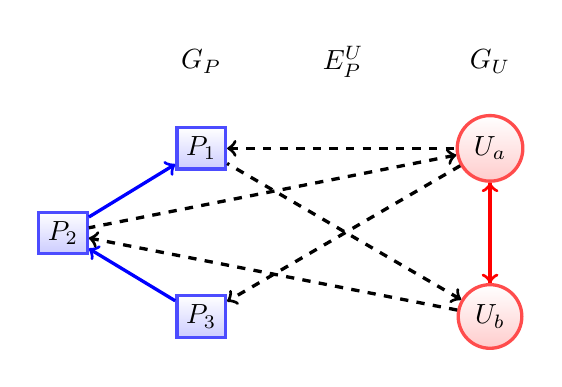
\begin{tikzpicture}[node distance=1em]
      \matrix[row sep=1em, column sep=3em] {
        & \node {$G_P$};& \node {$E_P^U$}; & \node {$G_U$};\\
        & \node (post_a) [post] {$P_1$}; & & \node (user_a) [user] {$U_a$};\\
        \node (comment_1) [post] {$P_2$}; & & & \\
        & \node (comment_2) [post] {$P_3$}; & &\node (user_b) [user] {$U_b$};\\
      };

      \path (post_a) edge[<-, blue, very thick] (comment_1)
            (comment_1) edge[<-, blue, very thick] (comment_2);

      \path (post_a) edge[<-, dashed, very thick] (user_a);
      \path (user_b) edge[<-, dashed, very thick] (post_a)
            (user_b) edge[->, dashed, very thick] (comment_1);
      \path (user_a) edge[<-, dashed, very thick] (comment_1)
            (user_a) edge[->, dashed, very thick] (comment_2);

      \path (user_a) edge[<-, red, very thick] (user_b)
            (user_a) edge[->, red, very thick] (user_b);
    \end{tikzpicture}
    \label{fig:model:hypergraph}
  \end{figure}
  \pause
  Note that there are atleast 3 interesting graphs here. Where are they?
\end{frame}

\definecolor{litegreen}{HTML}{2ECC71}
\newcolumntype{h}{>{\columncolor{litegreen}}l}
\section{Case Study: \texttt{/r/uwaterloo}}
\begin{frame}[fragile]
  Applied centrality analysis to reveal the following top nodes,
  \begin{center}
    \begin{tabular}{h|l|l}
      \texttt{/r/uwaterloo}   & \texttt{/r/science} & \texttt{/r/CanadianInvestor} \\ \hhline{=|=|=}
      supersonic63            & t3\_7e1jo1          & johnnychi \\ \hline
      kw2002                  & AutoModerator       & EyesOnTsx\\ \hline
      \textbf{t3\_7f2c1d}              & mvea                & jnf\_goonie\\ \hline
      \textbf{t3\_7w0dgv}              & t3\_7vxito          & langlois44\\ \hline
      \textbf{t3\_7i045q}              & t3\_7s6a9z          & t3\_7ii8af\\ \hline
      microwavemasterrace     & t3\_7my58a          & t3\_7fapx7\\ \hline
      uwsmile                 & t3\_7okc7u          & t3\_7pawu6\\ \hline
      \textbf{t3\_7ld2jb}              & t3\_7hs6ro          & helkish\\ \hline
      mywaterlooaccount       & t3\_7sv8vb          & Ginhisf\\ \hline
      honhonhonFRFR           & t3\_7qs5xz          & MarketStorm
    \end{tabular}
  \end{center}
\end{frame}
\begin{frame}[fragile]
  \frametitle{Of Interest to \texttt{/r/uwaterloo}}
  \framesubtitle{The more generic submissions...}
  \begin{center}
    \begin{tabular}{r|l|c|c}
    Link & Description & Score & Comment \#\\ \hhline
    7f2c1d & Admissions Megathread & 311 & 12k \\ \hline
    7i045q & Mr. Goose for good exams... & 142 & 389 \\ \hline
    7ld2jb & Mr. Goose for good grades... & 196 & 371
    \end{tabular}
  \end{center}
  A mass thread on WaterlooWorks also shows up in the top 20.
\end{frame}
\begin{frame}[fragile]
  \frametitle{Of Interest to \texttt{/r/uwaterloo}}
  \framesubtitle{t3\_7w0dgv: A much more interesting post...}
  \begin{center}
    
\includegraphics[width=0.7\textwidth]{figures/7w0dgv}
  \end{center}
  \pause
  \begin{center}
    
\includegraphics[width=0.7\textwidth]{figures/davetompkins}
  \end{center}
\end{frame}

\section{General Observations}
\begin{frame}[fragile]
  \frametitle{General Observations}
  \framesubtitle{On \texttt{/r/science}}
  \begin{center}
    \begin{tabular}{l|h|l}
      \texttt{/r/uwaterloo}   & \texttt{/r/science} & \texttt{/r/CanadianInvestor} \\ \hhline{=|=|=}
      supersonic63            & \textbf{t3\_7e1jo1}          & johnnychi \\ \hline
      kw2002                  & AutoModerator       & EyesOnTsx\\ \hline
      t3\_7f2c1d              & mvea                & jnf\_goonie\\ \hline
      t3\_7w0dgv              & t3\_7vxito          & langlois44\\ \hline
      t3\_7i045q              & t3\_7s6a9z          & t3\_7ii8af\\ \hline
      microwavemasterrace     & t3\_7my58a          & t3\_7fapx7\\ \hline
      uwsmile                 & t3\_7okc7u          & t3\_7pawu6\\ \hline
      t3\_7ld2jb              & t3\_7hs6ro          & helkish\\ \hline
      mywaterlooaccount       & t3\_7sv8vb          & Ginhisf\\ \hline
      honhonhonFRFR           & t3\_7qs5xz          & MarketStorm
    \end{tabular}
  \end{center}
\end{frame}
\begin{frame}
  \frametitle{General Observations}
  \framesubtitle{On \texttt{/r/science}}
  \begin{center}
    
\includegraphics[height=0.8\textheight]{figures/7e1jo1}
  \end{center}
\end{frame}
\begin{frame}
  \frametitle{General Observations}
  \framesubtitle{On \texttt{/r/science}}
  \begin{center}
    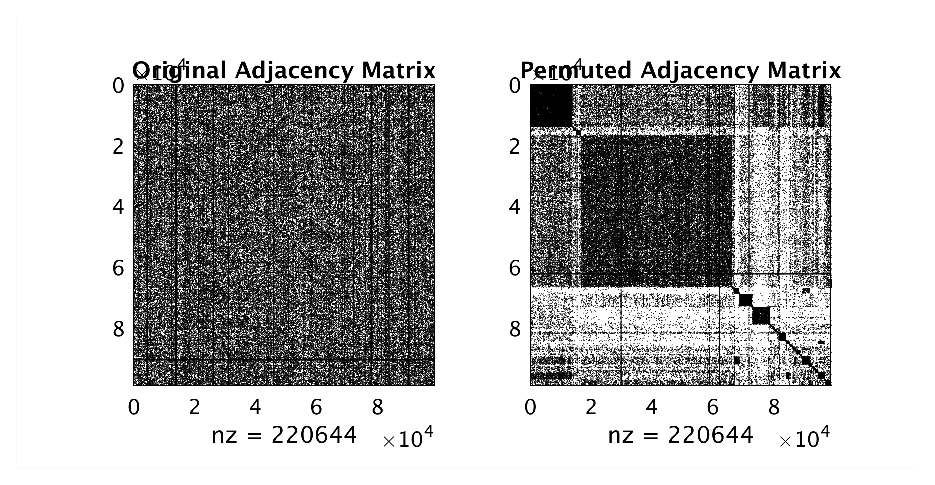
\includegraphics[width=\textwidth]{figures/science.eps}
  \end{center}
\end{frame}
\begin{frame}
  \frametitle{General Observations}
  \framesubtitle{On \texttt{/r/CanadianInvestor}}
  \begin{center}
    \begin{tabular}{l|l|h}
      \texttt{/r/uwaterloo}   & \texttt{/r/science} & \texttt{/r/CanadianInvestor} \\ \hhline{=|=|=}
      supersonic63            & t3\_7e1jo1          & johnnychi \\ \hline
      kw2002                  & AutoModerator       & EyesOnTsx\\ \hline
      t3\_7f2c1d              & mvea                & jnf\_goonie\\ \hline
      t3\_7w0dgv              & t3\_7vxito          & langlois44\\ \hline
      t3\_7i045q              & t3\_7s6a9z          & t3\_7ii8af\\ \hline
      microwavemasterrace     & t3\_7my58a          & t3\_7fapx7\\ \hline
      uwsmile                 & t3\_7okc7u          & t3\_7pawu6\\ \hline
      t3\_7ld2jb              & t3\_7hs6ro          & helkish\\ \hline
      mywaterlooaccount       & t3\_7sv8vb          & Ginhisf\\ \hline
      honhonhonFRFR           & t3\_7qs5xz          & MarketStorm
    \end{tabular}
  \end{center}
\end{frame}
\begin{frame}
  \frametitle{General Observations}
  \framesubtitle{On \texttt{/r/CanadianInvestor}}
  \begin{center}
    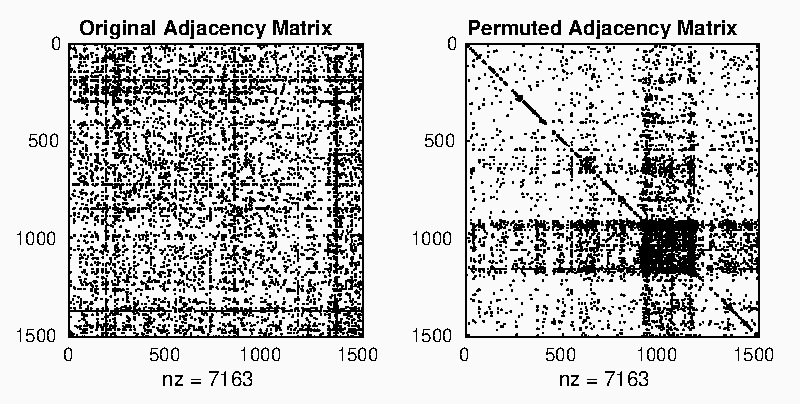
\includegraphics[width=\textwidth]{figures/CanadianInvestor.eps}
  \end{center}
\end{frame}

\section{Summary}
\begin{frame}
  \frametitle{Summary}
  \framesubtitle{What did we learn?}
  \begin{itemize}
    \item<1->{Infinity is odd.}
    \item<2->{Users totally read what they react to.}
    \item<3->{Dave Tompkins is awesome.}
    \item<4->{Obligatory reference to Trump.}
    \item<5->{Importance of investing expertise.}
  \end{itemize}
\end{frame}

\end{document}

